\chapter{Implementação}
\label{implementation-algorithm}

Neste capítulo serão apresentados detalhes da implementação deste trabalho. Será apresentada a arquitetura que foi criada para o desenvolvimento do algoritmo proposto, um diagrama de sequência, que proverá melhor visibilidade sobre os passos que são seguidos na sua execução e uma explicação sobre os elementos que o compõe.

\section{Arquitetura}

A Figura \ref{architecture} apresenta a arquitetura que foi utilizada para a realização dos experimentos. A arquitetura foi desenvolvida com o intuito de reproduzir uma aplicação real de um algoritmo de criptografia. As partes do cifrador e do decifrador são executadas em dois computadores distintos que se comunicam utilizando o protocolo de rede TCP/IP.

De maneira geral, cada lado terá uma \textit{thread} que auxiliará no envio/recebimento do \textit{byte} cifrado usando o \textit{socket} TCP/IP. A parte de cifração/decifração será utilizando o núcleo do \textit{RC4} alterado de forma a implementar o algoritmo de balanceamento proposto

\begin{figure}[h]
	\centering
	\includegraphics[scale=0.5]{figuras/architecture.eps}
	\caption{Arquitetura utilizada no projeto}
	\label{architecture}
\end{figure}

\subsection{Inicializador do Gerador}

Esse elemento é responsável por fazer a inicialização do gerador que será utilizado  no algoritmo.

O gerador escolhido para os experimentos foi o do próprio \textit{RC4}. O \textit{RC4} tem como entradas o texto em claro que será cifrado e uma chave, esta chave é utilizada para fazer a inicialização do gerador. A chave utilizada foi gerada pelo \textit{ssh-keygen}.

\subsection{Gerador de \textit{Bytes}}

Como explicado anteriormente, o gerador escolhido foi o do próprio \textit{RC4} e sua geração foi feita de acordo com o que o algoritmo aconselha. 


\subsection{Fila de Mensagem}

A fila de mensagem foi utilizada para servir de intermediário entre o cifrador/decifrador e a \textit{thread} que envia/recebe os \textit{bytes} cifrados. 
  
\subsection{\textit{Thread} de Envio para Decifrador}

Esta thread é responsável por retirar os bytes cifrados da fila de mensagens e os enviar, via \textit{TCP/IP}, para o decifrador.

Optou-se pelo uso desta \textit{thread} para minimizar o \textit{overhead} do envio dos bytes pela rede através da paralelização da execução,  evitando, com isso, que o cifrador fique parado aguardando a rede.
\subsection{\textit{Thread} para Receber do Cifrador}

Assim como no cifrador, o decifrador também conta com uma \textit{thread} auxiliar para receber os \textit{bytes} que são enviados pelo cifrador e escrever na fila de mensagem.

Neste caso, provavelmente, o uso da \textit{thread} não traz um ganho apreciável, visto que a rede é o maior gargalo, por isso, a leitura do \textit{socket} é feita a medida que o \textit{buffer} do \textit{TCP/IP} se completa.

\subsection{\textit{TCP/IP}}

Quando estávamos analisando o melhor protocolo de comunicação para ser utilizado em conjunto com o algoritmo, decidimos pelo TCP/IP pela reciprocidade que o mesmo contém,, além da garantia de entrega e sequência dos dados 

Em algoritmos de criptografia, a ordem com que os \textit{bytes} são enviados/lidos é de extrema importância, para que o texto decifrado tenha consistência e integridade. 
\subsection{Decifrador}

Processo responsável em fazer a tradução dos \textit{bytes} cifrados. 

O decifrador irá ter acesso aos \textit{bytes} cifrados na fila de mensagem que será populada pela \textit{thread} de recebimento. A operação que é efetuada é somente um ou-exclusivo do \textit{byte} proveniente do gerador e o \textit{byte} correspondente.

\subsection{Cifrador}

Processo responsável em cifrar os \textit{bytes} em claro que se deseja obter segurança.

Uma vez cifrado, postará na fila de mensagens para que a \textit{thread} de envio faça a sua parte e envie o mesmo para o decifrador

\section{Diagrama de Sequência}

O diagrama de sequência representado na Figura \ref{sequence-diagram} tem como objetivo demonstrar como os processos,cifra e  decifra, interagem com os outros elementos, tais como: fila de mensagem, \textit{threads} e a comunicação entre os mesmos. 

\begin{figure}[h]
	\centering
	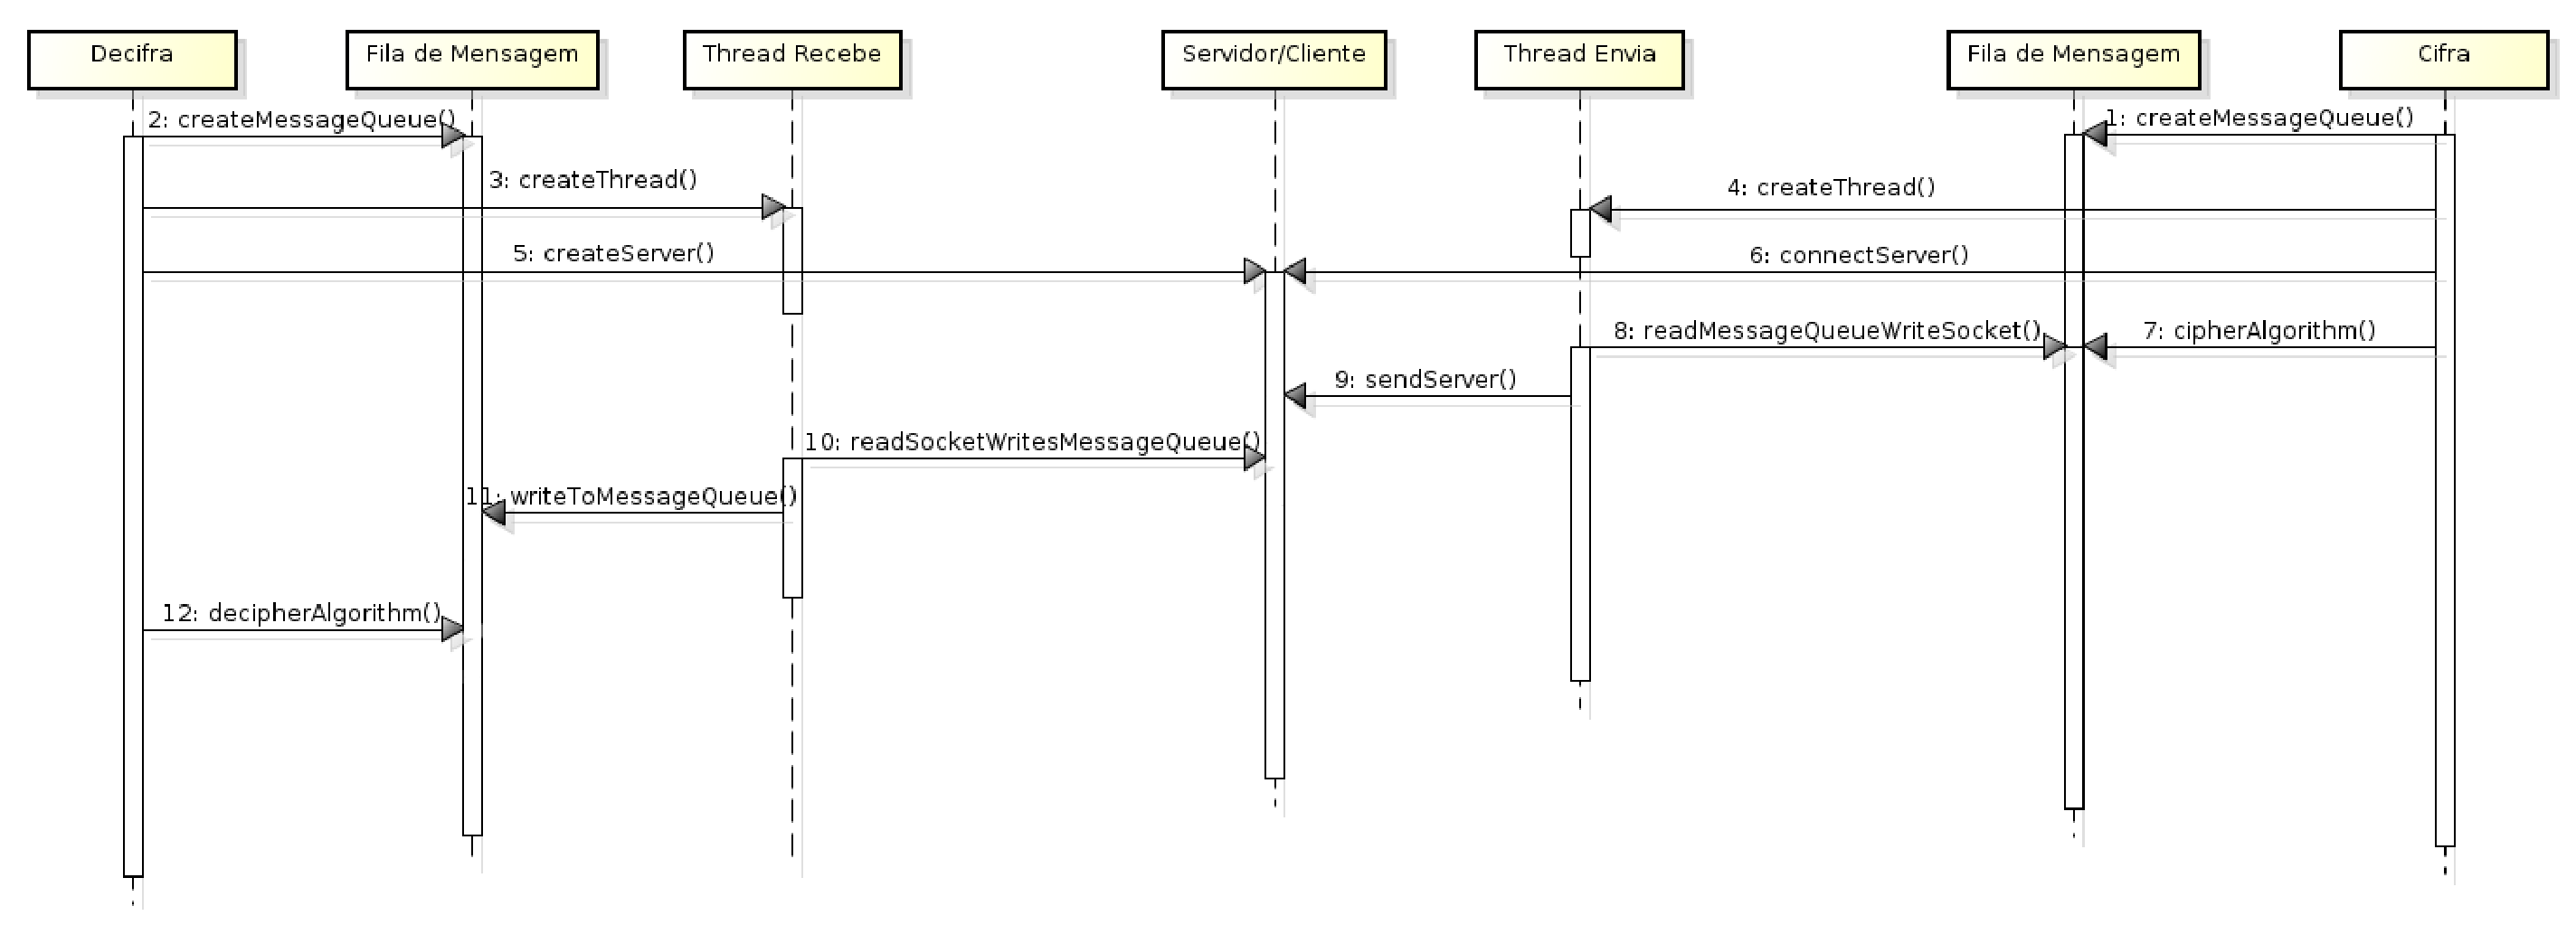
\includegraphics[scale=0.5, angle = 90]{figuras/sequenceDiagram.eps}
	\caption{Diagrama de Sequência}
	\label{sequence-diagram}
\end{figure}


\begin{enumerate}
	\item O processo de decifração deve ser o primeiro a ser iniciado, pois ele é responsável por iniciar o servidor em que o processo da cifra irá se conectar para a comunicação e envio de \textit{bytes} cifrados.
	\item Em seguida, o processo de decifração irá iniciar a \textit{thread} que será responsável por ler as mensagens proveniente do \textit{socket} de comunicação.
	\item O processo de decifração também inicia a fila de mensagem que irá utilizar.
	\item Quando o processo de cifração inicia, ele tenta se conectar com o servidor e o servidor o aceita ou não.
	\item Quando a comunicação é estabelecida, o processo de cifração inicia a \textit{thread} que será responsável por enviar os \textit{bytes} cifrados para o decifrador.
	\item Por fim, o processo de cifração também inicia a fila de mensagem.
	\item Os passos anteriores são somente para inicialização dos processos e \textit{threads}. A parte de cifração começa quando tudo já está iniciado e acontece da seguinte forma:
		\begin{enumerate}
			\item O processo de cifração faz a leitura do arquivo que contém o texto em claro e junto com o \textit{byte} do gerador executa a operação de ou-exclusivo.
			\item Em seguida, o \textit{byte} cifrado é postado na fila de mensagem.
			\item Por sua vez, a \textit{thread} que envia os \textit{bytes} cifrados, faz a leitura da fila de mensagem e envia para o decifrador o \textit{byte} cifrado.
			\item A \textit{thread} que faz a leitura do \textit{socket}, recebe o valor do \textit{byte} cifrado e o escreve na fila de mensagem do decifrador.
			\item Por fim, o decifrador faz a leitura da fila de mensagem e o decifra realizando a operação ou-exclusivo com o \textit{byte} do gerador.
		\end{enumerate}

\end{enumerate}
